%-------------------------------------------------------------------------------------
\section{Experiment on Single Conditional Distribution}

We also did some experiments for three-dimensional synthetic data that each view has the same conditional distribution. We generated the data from two settings:
\begin{itemize}
\item[1.] Mixture of Gaussian conditional density;
\item[2.] Mixture of Gaussian and shifted Gamma conditional density.
\end{itemize}
The mixture proportion and other experiment settings are exact same as the experiment in the main text. The only difference is that the conditional densities for each view here are the identical. We use the same measure to evaluate the performance. The empirical results are plotted in Figure~\ref{fig:sym_case}.

\begin{figure*}[!t]
%   \centering
  \renewcommand{\tabcolsep}{1pt}
  \begin{tabular}{cccc}
    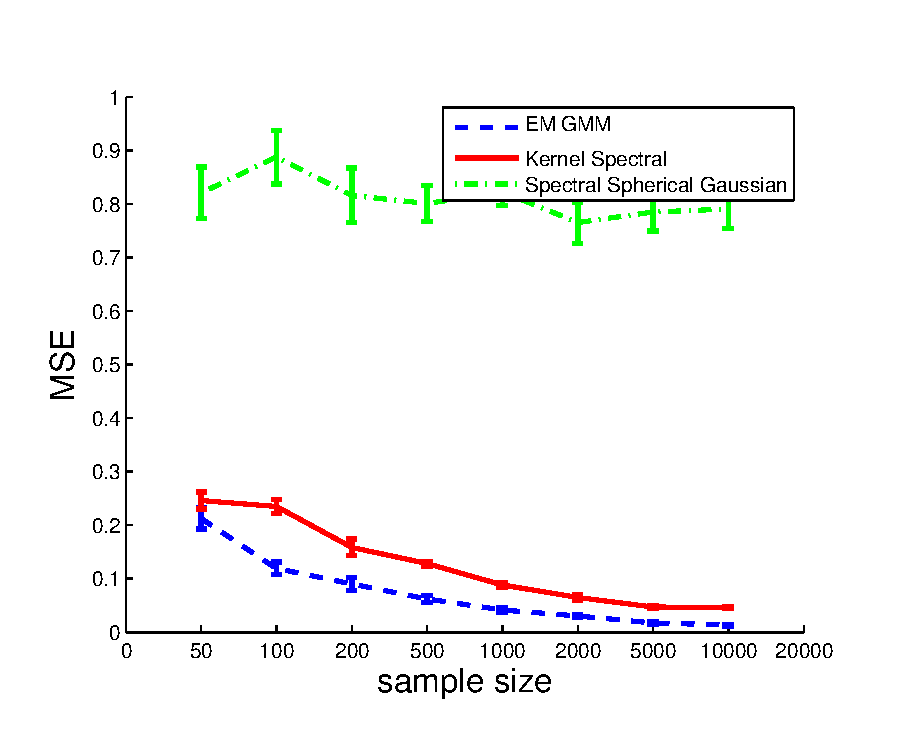
\includegraphics[width=0.26\textwidth]{../experiment/figure/sp_sym_gauss_k_2} &      
    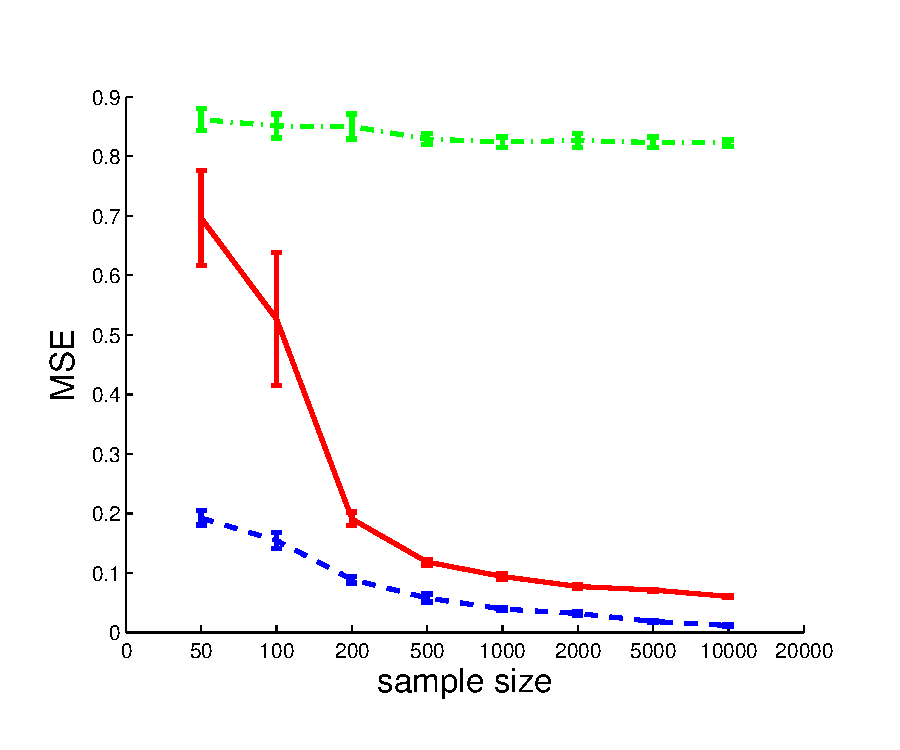
\includegraphics[width=0.26\textwidth]{../experiment/figure/sp_sym_gauss_k_3} &      
    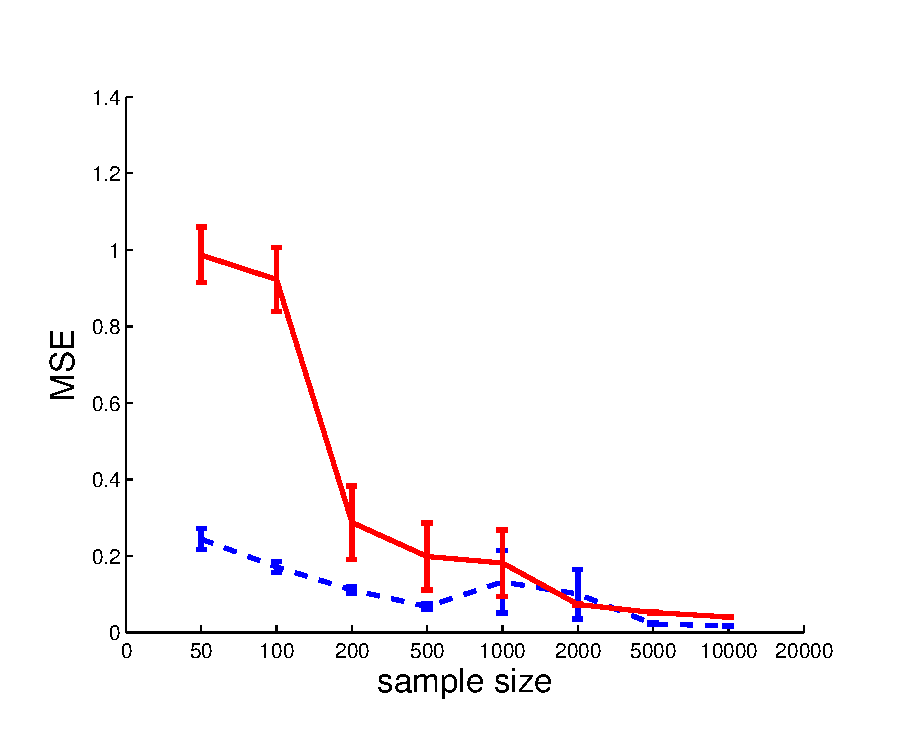
\includegraphics[width=0.26\textwidth]{../experiment/figure/sp_sym_gauss_k_4} &    
    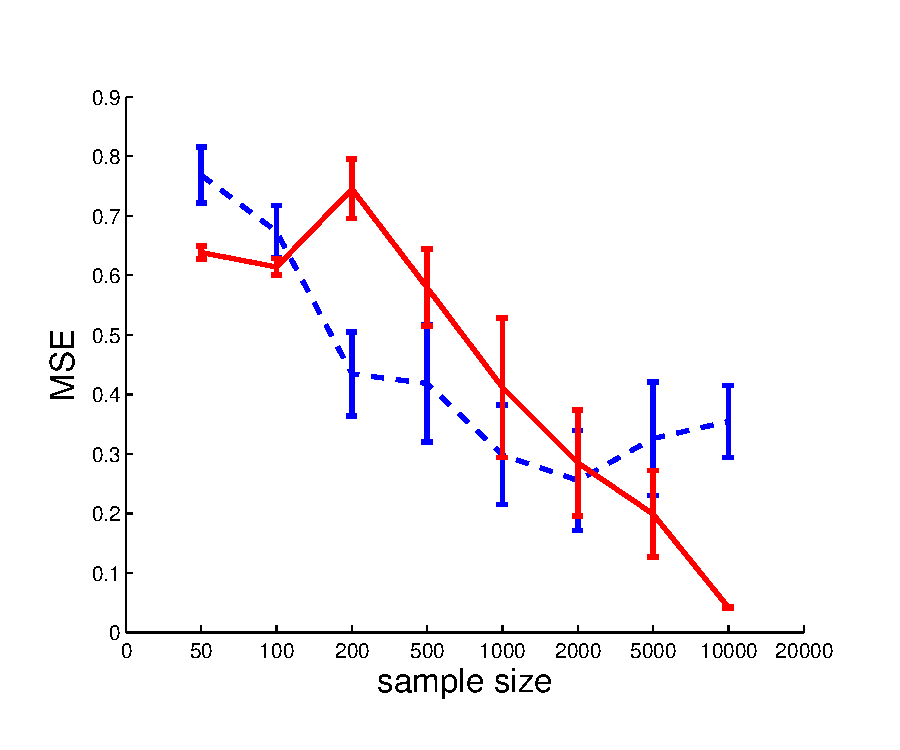
\includegraphics[width=0.26\textwidth]{../experiment/figure/sp_sym_gauss_k_8} \\    
    (a) Gaussian $k=2$ & (b) Gaussian $k=3$ & (c) Gaussian $k=4$ & (d) Gaussian $k=8$ \\ 
    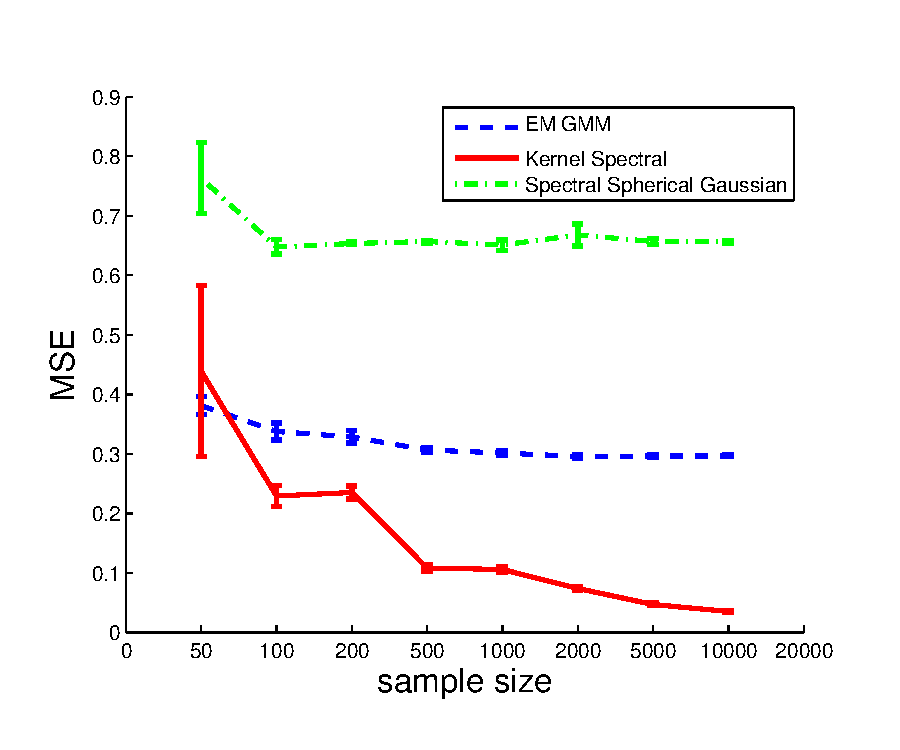
\includegraphics[width=0.26\textwidth]{../experiment/figure/sp_sym_heter_k_2} &      
    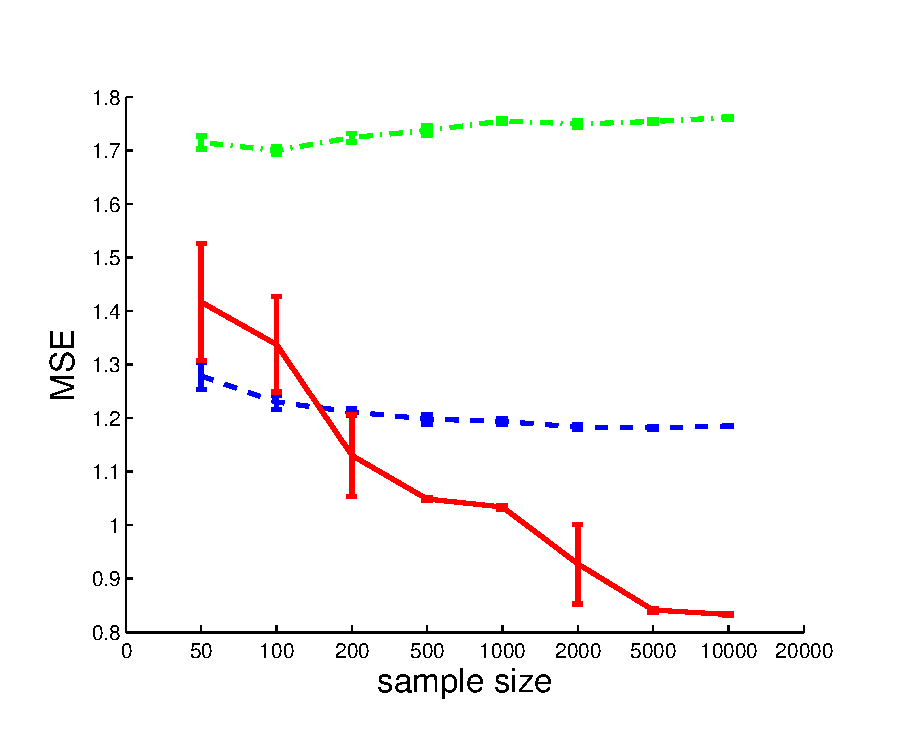
\includegraphics[width=0.26\textwidth]{../experiment/figure/sp_sym_heter_k_3} &      
    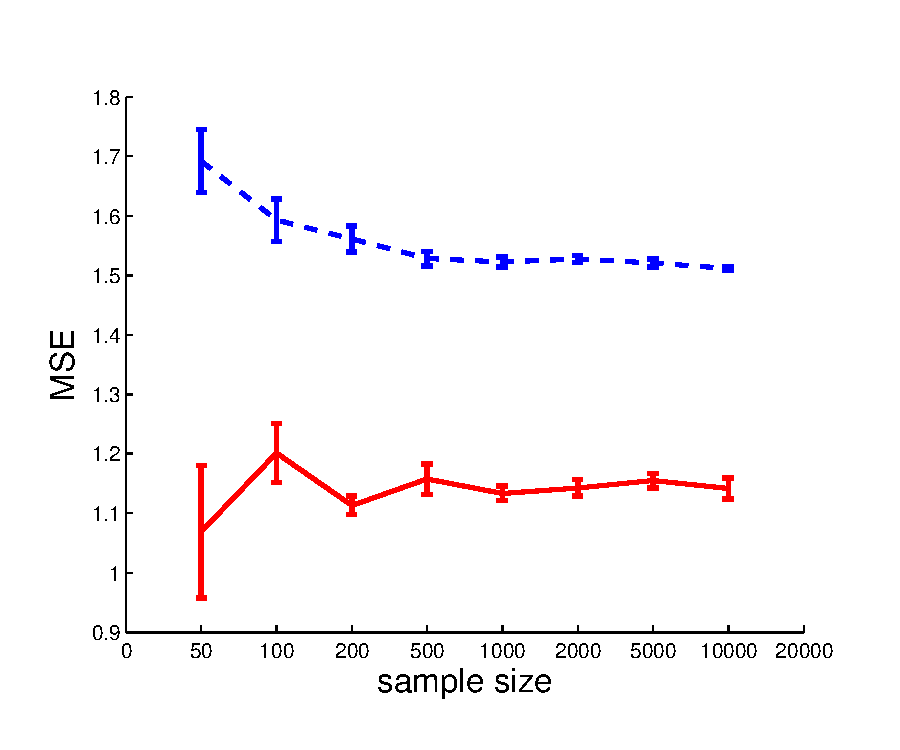
\includegraphics[width=0.26\textwidth]{../experiment/figure/sp_sym_heter_k_4} &    
    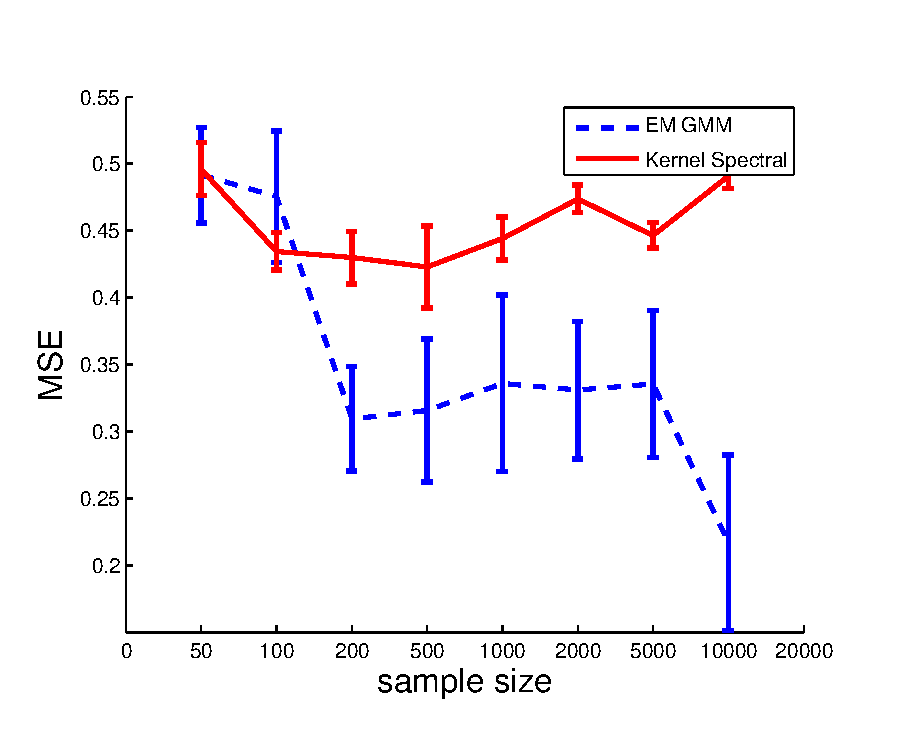
\includegraphics[width=0.26\textwidth]{../experiment/figure/sp_sym_heter_k_8} \\    
    (e) Gaussian/Gamma $k=2$ & (f) Gaussian/Gamma $k=3$ & (g) Gaussian/Gamma $k=4$ & (h) Gaussian/Gamma $k=8$ \\
  \end{tabular}
  \caption{(a)-(d) Mixture of Gaussian distributions with $k=2,3,4,8$ components. (e)-(h) Mixture of Gaussian/Gamma distribution with $k=2,3,4,8$. For the former case, the performance of kernel spectral algorithm converge to those of EM algorithm for mixture of Gaussian model. For the latter case, the performance of kernel spectral algorithm are consistently much better than EM algorithm for mixture of Gaussian model. Spherical Gaussian spectral algorithm does not work for $k=4,8$, and hence not plotted.}\label{fig:sym_case}
\end{figure*}

As we expected, the behavior of the proposed method is similar to the results in different conditional densities case. In mixture of Gaussians, our algorithm converges to the EM GMM resuls. And in the mixture of Gaussian/shift Gamma, our algorithm consistently better to other alternatives. 
